\section{Question 1}
\subsection{Finding the Equilibria}
\label{sec:equilibria}
%find equilibria
The first step that needs to taken to analyse the dynamics and find the bifurcation is to find the equilibria. This is done by setting all derivatives of q equal to 0, and finding the nullclines. Using the supplied equation the result is:

\begin{equation}\label{eq:rootfinder}Kq + N(q) = 0,\end{equation}

\noindent This can also be shown as: \\ 


\begin{equation} \begin{pmatrix}
  k\omega _0 & 2\pi\rho b U^{2} \\
  0 & k\alpha _{0}-2\pi(\frac{1}{2}  + a)\rho b^{2}U^{2}
  \end{pmatrix}
  \begin{pmatrix}
  h \\
  \alpha 
  \end{pmatrix} + 
  \begin{pmatrix}
  0 \\
  k_{\alpha 1}\alpha ^{2} +  k_{\alpha 2}\alpha ^{3}
  \end{pmatrix} = 0
  \label{eq:equilibmatrix}
  \end{equation}\\
  
\noindent From expanding this matrix, two equations can be found. These can then be simplified to find a linear equation of $h$ and $\alpha$, and a cubic equation of $\alpha$. The equilibria are found to be:

\begin{equation}\label{eqn:equilibrium1}
For\; \alpha = 0,  \; \;h = 0, \end{equation}\\
\begin{equation}\label{eqn:equilibrium2}
For \:\alpha = \frac{-k_{\alpha_{1}}\pm \sqrt{k_{\alpha_{1}}^{2} - 4\cdot k_{\alpha_{2}}\cdot k_{\alpha_{0}}}}{2k_{\alpha_{2}}}
\end{equation}

\begin{equation}
\label{eqn:hequilibrium2}
h = \frac{-2\pi \rho b U^{2} \alpha}{k_{\omega_{0}}}
\end{equation}

\noindent As can be seen from Equation \ref{eqn:equilibrium1} and Equations \ref{eqn:equilibrium2} and \ref{eqn:hequilibrium2}, there are three equilibria, one at zero and two that are a complex conjugate pair. From this, it can be realised that there is a singular equilibrium at $\alpha, \:h = 0$ (the trivial solution, as there is no oscillation), as complex equilibria do not exist. The trivial solution is independent of $U$, meaning that it is constant throughout all changes in $U$.
%Math Mode the derivation of equilibria
%Talk about how the complex equilibria aren't there

\subsection{The Jacobian}
\label{sec:jacobian}
Using the Jacobian matrix, which is calculated from the partial derivatives of the system equation in state-space form, it is possible to identify the stability of the system. For the trivial solution ($\alpha , h = 0$), the Jacobian is the linear parts of the state-space equations i.e, the nonlinear terms have no effect on it. This is because the only equilibrium is at $h, \alpha = 0$, and the nonlinear terms are functions of $h$ and $\alpha$.
Using Matlab, is is possible to find the eigenvalues of the Jacobian for $U$ from 0 to 50. These eigenvalues dictate the stability of the system. \\

\begin{equation}
\label{eqn:eigeneqn}
U(t) = Q\mathrm{e}^{\lambda t}Q^{-1}U_{0}
\end{equation}\\

\noindent In order to analyse the stability of the system, Equation \ref{eqn:eigeneqn} is used, where $Q$ is the eigenvectors of the linearisation of the system (in this example, the Jacobian), $\lambda$ is the eigenvalues and $U_{0}$ is the initial conditions. This equation shows that the system response ($U(t)$) is dependent on the eigenvalues of the Jacobian, or more precisely on $e^{\lambda t}$. This means that the higher the real part of the eigenvalue, the more effect it will have on the stability of the system. So only the higher eigenvalues need to be taken in to consideration for the stability. This dominant part is the right side of Figure \ref{fig:realeigu}.

%Show graph of the eigenvalues
\subsubsection{Stability}
\begin{figure}[H]
\centering
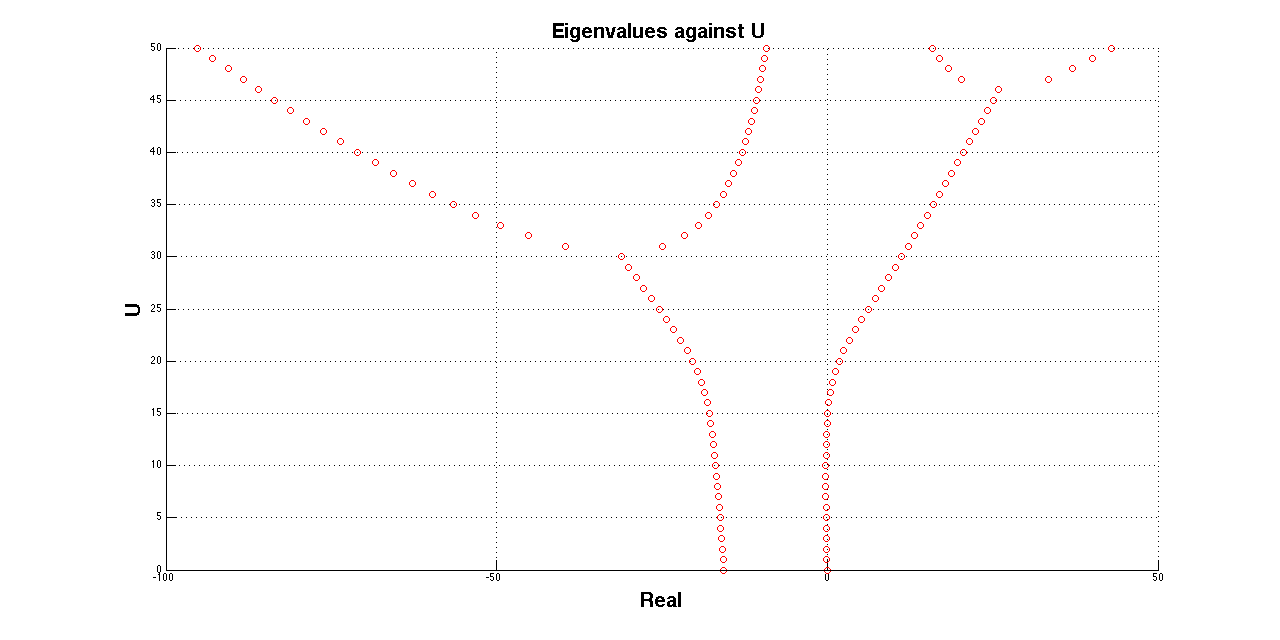
\includegraphics[width=1.0\textwidth]{realeigu.png}
\caption{\label{fig:realeigu} A plot of the real part eigenvalues against $U$, from $U = 0$ to $U=50$.  }
\end{figure}


%explain the stability of the system
\noindent From the eigenvalues from $U = 0$ to $U = 14$, (as shown in Figure \ref{fig:realeigu}) it can be seen that the system is a spiral attractor, as the eigenvalues are negative complex, and there is a decay towards the equilibrium (0) for both $h$ and $\alpha$. This is shown in Figure \ref{fig:k395attract}, where a small perturbation has been applied to the system and it returns to its equilibrium state. Then, as $U$ increases to between 14 and 15, it undergoes a bifurcation, as the real parts of the eigenvalues pass through the imaginary axis. Then, the system  becomes a spiral repeller, as the eigenvalues that affect it most (from Section \ref{sec:jacobian}) are complex with positive real parts. This is until $U= 47$, where the system then becomes a straight repeller, rather than a spiral, as the two eigenvalues with positive real parts then have no imaginary parts.\\  

\begin{figure}[H]
\centering
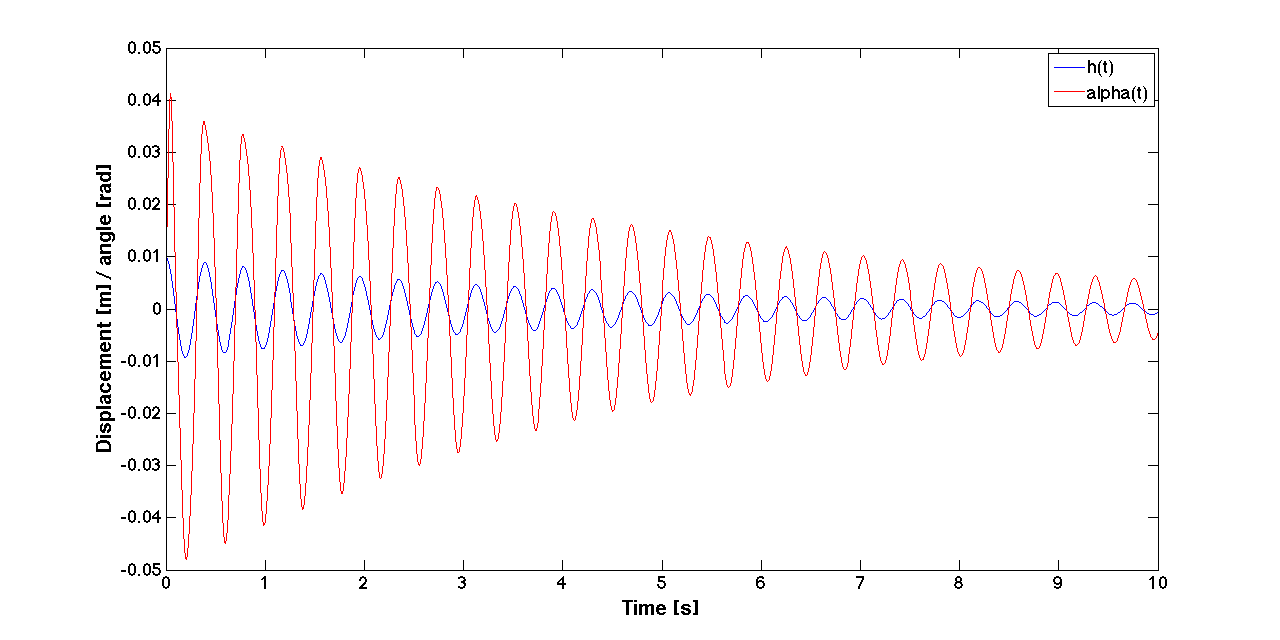
\includegraphics[width=1.0\textwidth]{k395attract.png}
\caption{\label{fig:k395attract} A plot of $h$ and $\alpha$ against $t$ showing how the system returns to its equilibrium at $U=10$ when a small perturbation is applied.  }
\end{figure}

\subsubsection{Bifurcation}
%What is the bifucation?
\noindent As was stated earlier, there is a bifurcation that occurs between $U=14$ and $U = 15$. This bifurcation can be found because in Figure \ref{fig:realeigu}, the point goes from one side of 0 to another. This signifies the crossing of the imaginary axis.
\noindent It is possible to classify the type of bifurcation that this is using the eigenvalues that were mentioned earlier. The eigenvalues found were a pair of negative real complex eigenvalues. These then cross the imaginary axis to become a set of positive real complex eigenvalues. As they are complex and cross the imaginary axis, this bifurcation is a Hopf bifurcation. \\
%Show where the bifurcation can be calculated from
\begin{figure}[H]
\centering
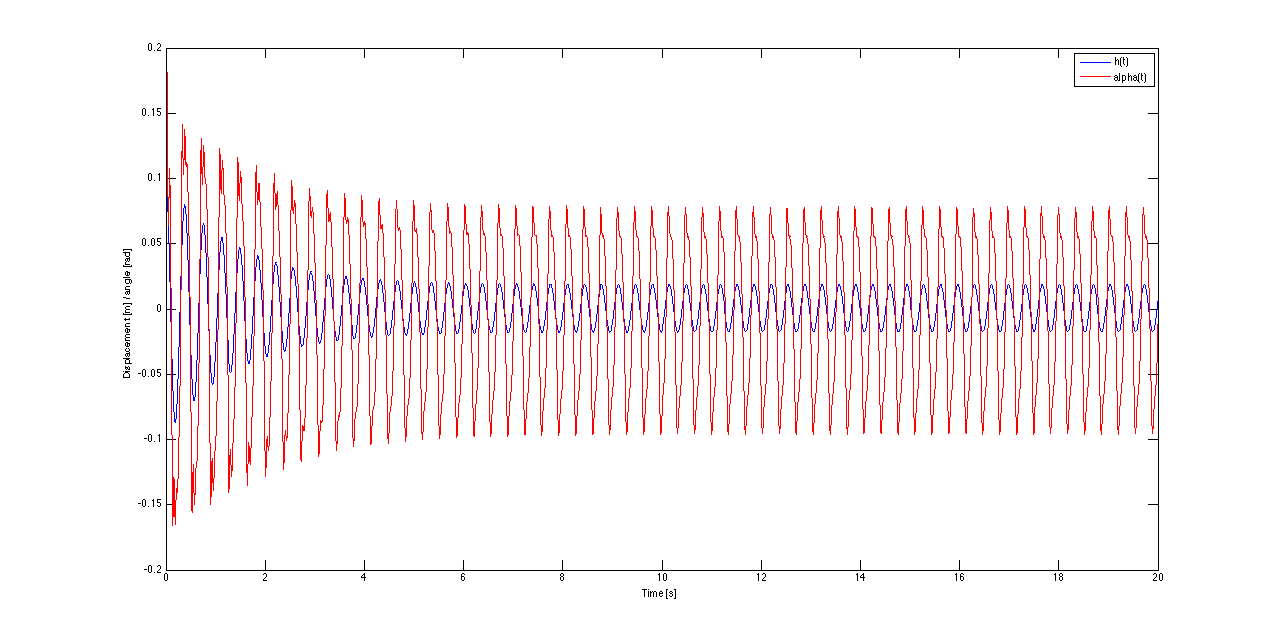
\includegraphics[width=1.0\textwidth]{limitcycle.png}
\caption{\label{fig:limitcycle} A plot of the change in $h$ and $\alpha$ against $t$. It shows the limit cycle as there is no drop off towards an equilibrium}
\end{figure}


\noindent A Hopf bifurcation is when a limit cycle (a periodic orbit) is created, as eigenvalues cross the imaginary axis. The limit cycle can be seen in Figure \ref{fig:limitcycle}. We can assume that the bifurcation is supercritical, as the limit cycle only occurs for $U>15$. This is where the aero-elastic flutter appears, as the periodic orbit is the motion the aerofoil undergoes. For $U<15$, there is a decay to the equilibrium at 0. 
%Bifurcation conditions?
%Hopf when the right side of the eigenvalue plot crosses 0
%limit cycles?
